\documentclass[a4paper,11pt]{book}
\renewcommand{\familydefault}{\sfdefault}

\usepackage{graphics} % for pdf, bitmapped graphics files
\usepackage{graphicx}
\usepackage{exsheets}
\usepackage{amsmath}
\usepackage{amssymb}
\usepackage{algorithm}
\usepackage{algorithmicx}
\usepackage[noend]{algpseudocode}
\usepackage{hyperref}
\usepackage{enumitem}
\usepackage{filecontents}
\usepackage{multirow}
\usepackage{tikz}
%\usepackage{showframe}% to show frames

\graphicspath{{images/}} 

\def\BState{\State\hskip-\ALG@thistlm}


\definecolor{TitleColor}{rgb}{0.65,0.04,0.07}
\definecolor{NumberColor}{rgb}{0.02,0.04,0.48}

\DeclareInstance{exsheets-heading}{fancy}{default}{
toc-reversed = true ,
indent-first = true ,
vscale = 2 ,
pre-code = \IfInsideQuestionT{\rule{\linewidth}{1pt}} ,
post-code =\IfInsideQuestionT{\rule{\linewidth}{1pt}} ,
subtitle-format = \large\scshape\color{rgb:red,0.65;green,0.04;blue,0.07} ,
number-format = \large\bfseries\color{rgb:red,0.02;green,0.04;blue,0.48} ,
points-format = \itshape ,
join = { number[r,B]title[l,B](.333em,0pt);
title[r,B]subtitle[l,B](1em,0pt)
} ,
attach =
{
main[hc,vc]number[hc,vc](0pt,0pt) ;
main[l,vc]subtitle[hc,vc](\marginparsep,0pt)
}
}



\DeclareInstance{exsheets-heading}{block-subtitle}{default}{
vscale = 2 ,
pre-code = \rule{\linewidth}{1pt} ,
post-code = \rule{\linewidth}{1pt} ,%title-format = \large\scshape\color{TitleColor} ,
number-format = \large\bfseries\color{rgb:red,0.02;green,0.04;blue,0.48} ,
subtitle-format = \large\scshape\color{black} ,
join = {
title[r,B]number[l,B](.333em,0pt) ;
title[r,B]subtitle[l,B](1em,0pt)
} ,
attach = {
main[l,vc]title[l,vc](0pt,0pt) ;
main[r,vc]points[l,vc](\marginparsep,0pt)
},
}

\DeclareQuestionClass{textbook}{textbooks}

\SetupExSheets{
  headings = fancy,
  question/print = true ,
  solution/print = true }
 % counter-format = se.qu ,
%  counter-within = section ,
  %question/pre-hook = \rule{\textwidth}{1pt},


\hypersetup{
	colorlinks = true, 
	breaklinks = true, 
	bookmarks = true,
	bookmarksnumbered = true,
	urlcolor = blue, 
	linkcolor = blue, 
	citecolor=blue,
	linktoc=page, 
	pdftitle={}, 
	pdfauthor={\textcopyright Author}, 
	pdfsubject={}, 
	pdfkeywords={}, 
	pdfcreator={pdfLaTeX}, % PDF Creator
	pdfproducer={IEEE} }


\usetikzlibrary{arrows}

\tikzset{
  treenode/.style = {align=center, inner sep=0pt, text centered,
    font=\sffamily},
  arn_n/.style = {treenode, circle, white, font=\sffamily\bfseries, draw=black,
    fill=black, text width=1.5em},% arbre rouge noir, noeud noir
  arn_r/.style = {treenode, circle, red, draw=red, 
    text width=1.5em, very thick},% arbre rouge noir, noeud rouge
  arn_x/.style = {treenode, rectangle, draw=black,
    minimum width=0.5em, minimum height=0.5em}% arbre rouge noir, nil
}



\makeatletter
\@addtoreset{question}{section}
\makeatother


\begin{document}
\author{Asem Alaa}

\title{Data Compression [SBE628] (Fall 2017):\\ Assignment}

\maketitle

\chapter*{Information Theory}


\begin{question}
Suppose that X is a random variable that takes on values from an M-letter alphabet. Show that \\
$ 0 \leq H(x) \leq \log_2(M) $

\end{question}
\begin{solution}
Since entropy maximized when all events are equally probable, i.e $p=\frac{1}{M}$ for all events: \\
\begin{equation}
\begin{aligned}
H_{max}(X) &= - \sum_{i=1}^{M} p_i \log_2( p_i )  \\
&= - \sum_{i=1}^{M} \frac{1}{M} \log_2( \frac{1}{M} ) \\
&= - \log_2( \frac{1}{M} ) \\
&= \log_2( M ) \\
\therefore 0 \leq H(x) \leq \log_2(M)
\end{aligned}
\end{equation}  
\end{solution}


\begin{question}
An experiment has 2 binary random variable outputs X \& Y, with
the shown joint probabxilities. Calculate the amount of
information gained, or expected, from knowing each of the
following:

\begin{table}[h]
\renewcommand{\arraystretch}{1.3}
\centering
\begin{tabular}{c||c|c}
\hline
\bfseries $X$ & \bfseries $Y$ & $P(X,Y)$\\
\hline\hline	
0 & 0 & 0.2 \\
0 & 1 & 0.1 \\
1 & 0 & 0.1 \\
1 & 1 & 0.6 \\
\hline
\end{tabular}
\end{table} 

\begin{enumerate}
\item $Y=1$
\item The value of X. 
\item The value of Y, given $X=0$.
\item The values of both X, Y.
\item The average common information between X and Y.
\end{enumerate}
\end{question}
\begin{solution}
\begin{enumerate}

\item $H(X|Y=1)=-(\frac{1}{7}
log_2(\frac{1}{7}) + \frac{6}{7}
log_2(\frac{6}{7}) = 0.59$
\item $H(Y|X)=-(0.3log_2(0.3) + 0.7log_2(0.7) = 0.88$. 
\item  $H(Y|X=0)=-(\frac{1}{3}
log_2(\frac{1}{3}) + \frac{2}{3}
log_2(\frac{2}{3}) = 0.918$
\item 0 (no information if values of X and Y are given).
\item \begin{equation}
\begin{aligned}
H(X) &= -(0.3log_2(0.3) + 0.7log_2(0.7) = 0.88\\
H(Y) &= -(0.3log_2(0.3) + 0.7log_2(0.7) = 0.88\\
H_{avrg}(X,Y) &= \frac{H(X)+H(Y)}{2} = 0.88 \text{ bits/source}.
\end{aligned}
\end{equation}

\end{enumerate}
\end{solution}


\begin{question}
\begin{table}[h]
\renewcommand{\arraystretch}{1.3}
\centering
\begin{tabular}{c||c|c|c}
\hline
\bfseries Symbol & \bfseries a & b & c\\
\hline\hline	
Probability & 0.25 & 0.25 & 0.5 \\
\hline
\end{tabular}
\end{table} 

A source emits iid symbols form the alphabet {a, b, \& c}, with the following probabilities. Calculate the entropy of that source. 
\end{question}
\begin{solution}
$H(X)= -( 0.5\log_2(0.5) + 0.25\log_2(0.25) + 0.25\log_2(0.25) = 1.5 \text{bits (0.1875 bytes)}$
\end{solution}

\begin{question}
\begin{table}[h]
\renewcommand{\arraystretch}{1.3}
\centering
\begin{tabular}{c|c|c|c}
\hline
 $P(X_{n-1}) /P(X_{n}) $ & a  & b  & c \\
a & 0.5 & 0.125 & 0.375 \\
b & 0.125 & 0.5 & 0.375\\
c & 0.125 & 0.125 & 0.75 \\
\hline
\end{tabular}
\end{table}

The probability of the current symbol, $X_n$, emitted from the previous source, is found to be related to the previous symbol, $X_{n-1}$, as shown in table. Recalculate the entropy of the source.

\end{question}
\begin{solution}
\begin{itemize}
\item $P(a) = 0.25$
\item $P(b) = 0.25$
\item $P(c) = 0.5$
\end{itemize}


\begin{equation}
\begin{aligned}
H_1(a) &= -( P(a|a)\log(P(a|a)) + P(b|a)\log(P(b|a)) + P(c|a)\log(P(c|a))\\
&= - (  0.5\log(0.5) + 0.125\log(0.125) + 0.375\log(0.375)) \\
&= \text{1.4 bits}  \\
H_1(b) &= ( P(a|b)\log(P(a|b)) + P(b|b)\log(P(b|b)) + P(c|b)\log(P(c|b))\\
&= - (  0.125\log(0.125) + 0.5\log(0.5) + 0.375\log(0.375)) \\
&= \text{1.4 bits} \\
H_1(c) &= ( P(a|c)\log(P(a|c)) + P(b|c)\log(P(b|c)) + P(c|c)\log(P(c|c))\\
&= - (  0.125\log(0.125) + 0.125\log(0.125) + 0.75\log(0.75)) \\
&= \text{1.06 bits} \\
\therefore H(X_n|X_{n-1}) &= P(a)H(a) + P(b)H(b) + P(c)H(c) \\
&= \text{1.23 bits (0.15375 bytes)}
\end{aligned}
\end{equation}

\end{solution}


\begin{question}
\begin{itemize}
\item $P(A) = 0.125$
\item $P(C) = 0.125$
\item $P(G) = 0.25$
\item $P(T) = 0.5$
\end{itemize}
The bases of a genomic sequence have the probabilities shown. Calculate the self-information of “C”, and the entropy of the sequence. 
\end{question}
\begin{solution}
$i(C) = -log(P(C)) = \text{3 bits}$ \\

\begin{equation}
\begin{aligned}
H(S) &= -( P(A)\log(P(A)) + P(G)\log(P(G)) + P(C)\log(P(C)) + P(T)\log(P(T)) \\ 
&= \text{1.75 bits}
\end{aligned}
\end{equation}
\end{solution}

\begin{question}
\begin{table}[h]
\renewcommand{\arraystretch}{1.3}
\centering
\begin{tabular}{c||c|c|c|c}
\hline
 $B_{n-1} \text{\textbackslash} B_{n} $ & A  & C  & G & T \\
 \hline\hline
A & 0.4 & 0.2 & 0.1 & 0.3 \\
C & 0.2 & 0.4 & 0.2 & 0.2 \\
G & 0.1 & 0.1 & 0.3 & 0.5 \\
T & 0.05&0.05 &0.275&0.625 \\
\hline
\end{tabular}
\end{table}

The probability of the any base, $B_n$, in the previous sequence, is found to be related to its previous base, $B_{n-1}$, by the probabilities given in the following table. Recalculate the entropy of the sequence.
Note: $P(A) = 0.125$, $P(C) = 0.125$, $P(G) = 0.25$, and $P(T) = 0.5$.

\end{question}
\begin{solution}
\begin{equation}
\begin{aligned}
H_1(A) &= - P(A|A)\log(P(A|A)) - P(C|A)\log(P(C|A)) \\
&- P(G|A)\log(P(G|A)) - P(T|A)\log(P(T|A)) \\
&=  -0.4\log(0.4)  -0.2\log(0.2) -0.1\log(0.1) -0.3\log(0.3)) \\
&= \text{1.846 bits}  \\
H_1(C) &= -( P(A|C)\log(P(A|C)) - P(C|C)\log(P(C|C)) \\
&- P(G|C)\log(P(G|C) - P(T|C)\log(P(T|C)) \\
&= - (  0.2\log(0.2) - 0.4\log(0.4) - 0.2\log(0.2)- 0.2\log(0.2)) \\
&= \text{1.922 bits}  \\
H_1(G) &= -P(A|G)\log(P(A|G)) - P(C|G)\log(P(C|G)) \\ 
&- P(G|G)\log(P(G|G) - P(T|G)\log(P(T|G)) \\
&= -0.1\log(0.1) - 0.1\log(0.1) - 0.3\log(0.3)- 0.5\log(0.5)) \\
&= \text{1.685 bits}  \\
H_1(T) &= -P(A|T)\log(P(A|T)) - P(C|T)\log(P(C|T)) \\
&- P(G|T)\log(P(G|T) - P(T|T)\log(P(T|T)) \\
&= -0.05\log(0.05) - 0.05\log(0.05) - 0.275\log(0.275)- 0.625\log(0.625) \\
&= \text{1.368 bits}  \\
\therefore H(X_n|X_{n-1}) &= P(A)H(A) + P(C)H(C) + P(G)H(G) + P(T)H(T) \\
&= \text{1.57625 bits (0.197 bytes)}
\end{aligned}
\end{equation}

\end{solution}




\chapter*{Decodability}

\begin{question}
Determine whether each of the following codes is uniquely decodable (UD), prefix, instantaneous, or near instantaneous:
\begin{enumerate}
\item \{0,01,11,111\}
\item \{0,01,110,111\}
\item \{0,10,110,111\}
\item \{1,10,110,111\}
\end{enumerate}
\end{question}

\begin{solution}

\begin{table}[h]
\renewcommand{\arraystretch}{1.3}
\centering
\begin{tabular}{c|c|c|c|c}
\hline
 Code & UD  & Prefix  & Intantaneous & Near-instantaneous \\
\{0,01,11,111\} & F & F & F & T \\
\{0,01,110,111\} & F & F & F & T \\
\{0,10,110,111\} & F & F & F & F \\
\{1,10,110,111\} & F & F & F & F \\
\hline
\end{tabular}
\end{table}
\end{solution}

\begin{question}
An alphabet of 7 symbols, had code lengths of 2, 2, 3, 3, 3, 3, \& 3 bits. Is this code uniquely decodable? Why?
\end{question}
\begin{solution}
No. \\
Reasons: \\
$K = - \sum_{i=1}^{l} 2^{-l} = 2 \times 2^{-2} + 5 \times 2^{-3} = 1.125$ \\
$ \therefore \text{ not UD } (K>1).$ \\

\end{solution}


\begin{question}
What the largest number is of symbols that can be coded using a ternary (i.e. 3 symbols) code, while the code length of each symbol does not exceed 3? Why?
\end{question}
\begin{solution}
The largest number is 27.\\
Reasons: using a 3 symbols for each code results in $3^3$ variants. 
\end{solution}



\begin{question}
14 symbols are coded using a ternary (i.e. 3) code. The code lengths are 2, 2, 2, 2, 2, 2, 3, 3, 3, 3, 3, 3, 3, \& 3. Is this code uniquely decodable? Why?
\end{question}
\begin{solution}
Uniquely decodable. \\
Reasons: \\
$K = - \sum_{i=1}^{l} 3^{-l} = 6 \times 3^{-2} + 8 \times 3^{-3} = 0.963$ \\
$\therefore \text{ is decodable } (K<1)$.
\end{solution}


\begin{question}
An alphabet of 7 symbols, had code lengths of 2, 2, 3, 3, 3, 3, \& 3 bits. Is this code uniquely decodable? Why?
\end{question}
\begin{solution}
Not UD. \\
Reasons: \\
$K = - \sum_{i=1}^{l} 2^{-l} = 2 \times 2^{-2} + 5 \times 2^{-3} = 1.125$ \\
$ \therefore \text{ not UD } (K>1).$ \\

\end{solution}


\begin{question}
Using Kraft’s Inequality, check the decidability of the
following code table. Next, check the code table. Is the
code decodable? Why? Calculate the entropy, the average
code length, and the redundancy
\begin{table}[h]
\renewcommand{\arraystretch}{1.3}
\centering
\begin{tabular}{c|c|c}
\hline
Symbol & Probability & Code \\
a & 0.125 & 0 \\
b & 0.125 & 10 \\
c & 0.25 & 110 \\
d & 0.5 & 101 \\
\hline
\end{tabular}
\end{table}

\end{question}
\begin{solution}
Kraft’s inequality result: \\
$K = - \sum_{i=1}^{l} 2^{-l} = 2 \times 2^{-3} + 2^{-2} + 2^{-1} = 1$ \\
Decodability based on Kraft’s inequality: UD ($K\leq1$).\\
Is the code decodable? \\ 
No. \\
Why? \\
Dangling Suffixes = \{1,10,0\} which includes codes \{10,0\} from the original codes.\\
Average Code Length = 2.625 bits/symbol. \\
Redundancy = 0.875 bits/symbol.
\end{solution}


\begin{question}
Assume a 5-symbol alphabet \{A, B, C, D, E\}. Build a prefix code for the symbols. Then code the sequence: CBABAA.
\end{question}
\begin{solution}
\begin{table}[h]
\renewcommand{\arraystretch}{1.3}
\centering
\begin{tabular}{c|c|c|c|c|c}
\hline
Symbol & A & B & C & D & E \\
Code & 0 & 10 & 110 & 1110 & 1111 \\
\hline
\end{tabular}
\end{table}

\begin{table}[h]
\renewcommand{\arraystretch}{1.3}
\centering
\begin{tabular}{c|c|c|c|c|c|c}
\hline
Symbol & C & B & A & B & A & A \\
Code & 110 & 10 & 0 & 10 & 0 & 0 \\
\hline
\end{tabular}
\end{table}

\end{solution}




\chapter*{Huffman Coding}
\begin{question}
Design each of the following codes, and then calculate its average coding length, and
redundancy, per symbol.
\begin{enumerate}
\item A minimum variance Huffman code for the alphabet \{A, B, C, D\}, with probabilities, 0.1, 0.2, 0.3, \& 0.4, respectively.
\item A minimum variance extended Huffman code for the binary alphabet {0, 1}, with
probabilities 0.1 and 0.9, respectively. Generate a code word for every block of 3 symbol.
\item A 3-bit Tunstall code for the above binary alphabet.
\end{enumerate}
\end{question}
\begin{solution}

\begin{tabular}{||c|c||c|c||c|c||c|c||}
\hline 
\multicolumn{2}{||c||}{Min-Var Huffman} & \multicolumn{2}{||c||}{Huffman} & \multicolumn{2}{||c||}{Extended Huffman} & \multicolumn{2}{||c||}{Tunstall} \\ 
\hline 
Symbol & Code & Symbol & Code & Symbol & Code & Symbol & Code \\ 
\hline 
A & 011 & A & 001 & 000 & 11111 & 0 & 000 \\ 
\hline 
B & 010 & B & 000 & 001 & 11110 & 10 & 001 \\ 
\hline 
C & 00 & C & 01 & 010 & 11101 & 110 & 010 \\ 
\hline 
D & 1 & D & 1 & 011 & 11100 & 1110 & 011 \\ 
\hline 
• & • & • & • & 100 & 110 & 11110 & 100 \\ 
\hline 
• & • & • & • & 101 & 101 & 111110 & 101 \\ 
\hline 
• & • & • & • & 110 & 100 & 1111110 & 110 \\ 
\hline 
• & • & • & • & 111 & 0 & 1111111 & 111 \\ 
\hline 
$L_{ave}$ & 1.9  & $L_{ave}$ & 1.9  & $L_{ave}$ & 0.53 & $L_{ave}$ & 0.86  \\ 
\hline 
Red & 0.06 & Red & 0.06 & Red & 0.07 & Red & 0.4  \\ 
\hline 

\end{tabular} 

\end{solution}

\begin{question}
An alphabet is composed of the 6 symbols \{A, C, N, T, Y, $\Delta$\}. Design a minimum length code for the alphabet. Assign short codes for small index symbols. Use this code as a starting code during next problems.
\end{question}

\begin{solution}
\begin{tikzpicture}[level 1/.style={sibling distance=4cm},level 2/.style={sibling distance=2.5cm},level 3/.style={sibling distance=1cm}]
	\node {Root}
		child { node {0}
            child {node{0} 
                child{ node{0(A)}} 
                child{ node{1(C)}}}
			child {node{1}
			    child{ node{0(N)}} 
                child{ node{1(T)}}}		
		}
		child { node {1}
		    child{ node{0(Y)}} 
            child{ node{1($\Delta$)}}}		 		
	;
\end{tikzpicture}

\begin{tabular}{|c|c|}
\hline 
Symbol & Code \\ 
\hline 
A & 000 \\ 
\hline 
C & 001 \\ 
\hline 
N & 010 \\ 
\hline 
T & 011 \\ 
\hline 
Y & 10 \\ 
\hline 
$\Delta$ & 11 \\ 
\hline 
\end{tabular} 
\end{solution}

\begin{question}
Using adaptive Huffman coding,
\begin{enumerate}
\item code the following: “ACACTAN”. Show the development of the coding tree, and the code generated for each symbol.
\item Decode the first 5 symbols of the same alphabet, form the stream
“0111011001011001101100001111011000101001100011010101”
\end{enumerate}
\end{question}
\begin{solution}
\begin{enumerate}
\item Alphabet = \{A,C,N,T,Y,$\Delta$\} \\
$6=2^e + r$ \\
$e=2$ \\
$r=2$ \\
$\text{\#nodes}= 11$ \\
Initial codes: \\
\begin{tabular}{|c|c|}
\hline 
Symbol & Code \\ 
\hline 
A & 000 \\ 
\hline 
C & 001 \\ 
\hline 
N & 010 \\ 
\hline 
T & 011 \\ 
\hline 
Y & 10 \\ 
\hline 
$\Delta$ & 11 \\ 
\hline 
\end{tabular} 

\begin{itemize}
\item Code A = Code(NYT):Code(A). Transmit 000. \\
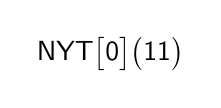
\begin{tikzpicture}[level 1/.style={sibling distance=4cm},level 2/.style={sibling distance=2.5cm},level 3/.style={sibling distance=1cm}]
	\node {NYT\big[0\big]\big(11\big)}		 		
	;
\end{tikzpicture}


\item Code C = Code(NYT):Code(C). Transmit 0001. \\
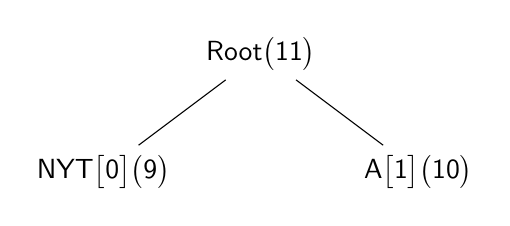
\begin{tikzpicture}[level 1/.style={sibling distance=4cm},level 2/.style={sibling distance=2.5cm},level 3/.style={sibling distance=1cm}]
	\node {Root\big(11\big)}
		child { node {NYT\big[0\big]\big(9\big)}}
        child { node {A\big[1\big]\big(10\big)}}	 		
	;
\end{tikzpicture}
\item Code A = 1. Transmit 1. \\
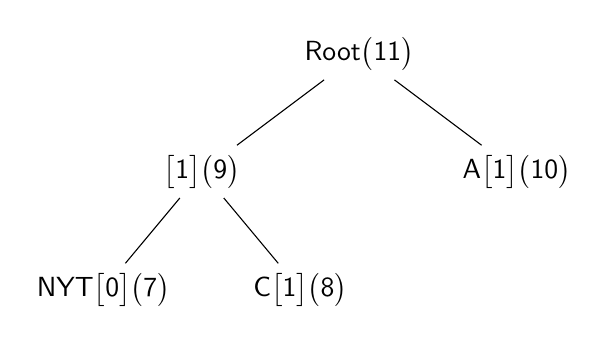
\begin{tikzpicture}[level 1/.style={sibling distance=4cm},level 2/.style={sibling distance=2.5cm},level 3/.style={sibling distance=1cm}]
	\node {Root\big(11\big)}
		child { node {\big[1\big]\big(9\big)} 
                child{ node{NYT\big[0\big]\big(7\big)}} 
                child{ node{C\big[1\big]\big(8\big)}}}
		child {node{A\big[1\big]\big(10\big)}}	
	;
\end{tikzpicture}
\item Code C = 01. Transmit 01. \\
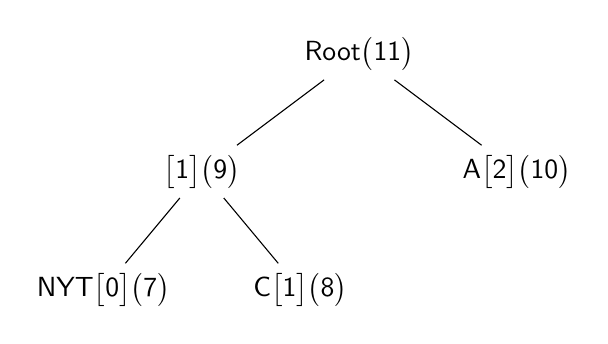
\begin{tikzpicture}[level 1/.style={sibling distance=4cm},level 2/.style={sibling distance=2.5cm},level 3/.style={sibling distance=1cm}]
	\node {Root\big(11\big)}
		child { node {\big[1\big]\big(9\big)} 
                child{ node{NYT\big[0\big]\big(7\big)}} 
                child{ node{C\big[1\big]\big(8\big)}}}
		child {node{A\big[2\big]\big(10\big)}}	
	;
\end{tikzpicture}
\item Code T = Code(NYT):Code(T). Transmit 00011. \\
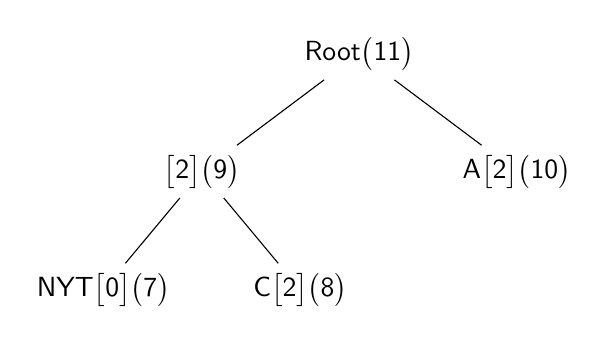
\begin{tikzpicture}[level 1/.style={sibling distance=4cm},level 2/.style={sibling distance=2.5cm},level 3/.style={sibling distance=1cm}]
	\node {Root\big(11\big)}
		child { node {\big[2\big]\big(9\big)}  
                child{ node{NYT\big[0\big]\big(7\big)}} 
                child{ node{C\big[2\big]\big(8\big)}}}
        child {node{A\big[2\big]\big(10\big)}}	
	;
\end{tikzpicture}
\item Code A = 1. Transmit 1. \\
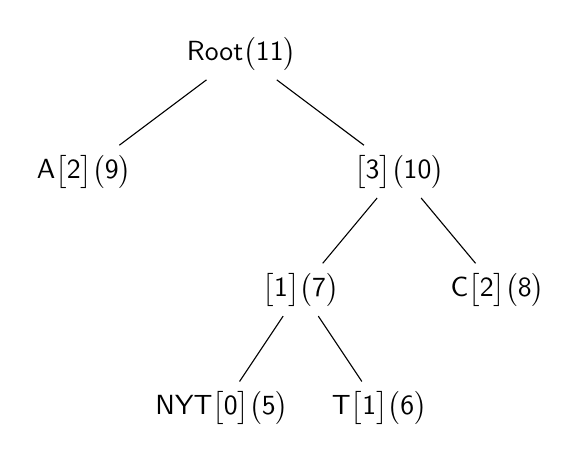
\begin{tikzpicture}[level 1/.style={sibling distance=4cm},level 2/.style={sibling distance=2.5cm},level 3/.style={sibling distance=2cm}]
	\node {Root\big(11\big)}
		child {node{A\big[2\big]\big(9\big)}}	
		child { node {\big[3\big]\big(10\big)}  
                child{ node{\big[1\big]\big(7\big)}
                        child{ node{NYT\big[0\big]\big(5\big)}} 
                        child{ node{T\big[1\big]\big(6\big)}}
                     } 
                child{ node{C\big[2\big]\big(8\big)}}
              }
               
	;
\end{tikzpicture}
\item Code N = Code(NYT):Code(N). Transmit 1000010.\\
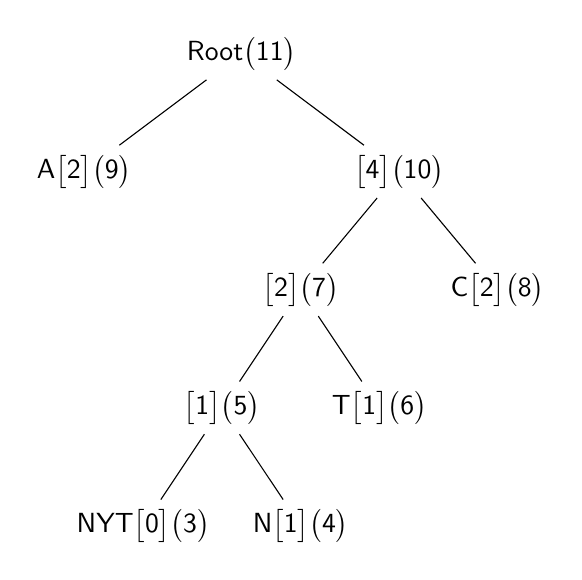
\begin{tikzpicture}[level 1/.style={sibling distance=4cm},level 2/.style={sibling distance=2.5cm},level 3/.style={sibling distance=2cm}]
	\node {Root\big(11\big)}
		child {node{A\big[2\big]\big(9\big)}}	
		child { node {\big[4\big]\big(10\big)}  
                child{ node{\big[2\big]\big(7\big)}
                        child{ node{\big[1\big]\big(5\big)} 
                                child{  node{NYT\big[0\big]\big(3\big)}}
                                child{  node{N\big[1\big]\big(4\big)}}
                             } 
                        child{ node{T\big[1\big]\big(6\big)}}
                     } 
                child{ node{C\big[2\big]\big(8\big)}}
              }
               
	;
\end{tikzpicture}
\end{itemize}
\item Decode “0111011001011001101100001111011000101001100011010101”.
\begin{itemize}
\item Encode 011 = T, then encode 1 = T, then encode 011=NYT+$\Delta$. \\
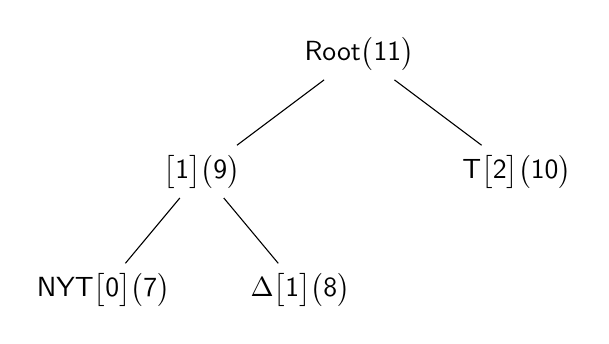
\begin{tikzpicture}[level 1/.style={sibling distance=4cm},level 2/.style={sibling distance=2.5cm},level 3/.style={sibling distance=2cm}]
	\node {Root\big(11\big)}
		child { node {\big[1\big]\big(9\big)}  
                child{ node{NYT\big[0\big]\big(7\big)}}
                child{ node{$\Delta$\big[1\big]\big(8\big)}}
              }
         child {node{T\big[2\big]\big(10\big)}}	
	;
\end{tikzpicture}
\item Encode 0010 = NYT+Y. \\
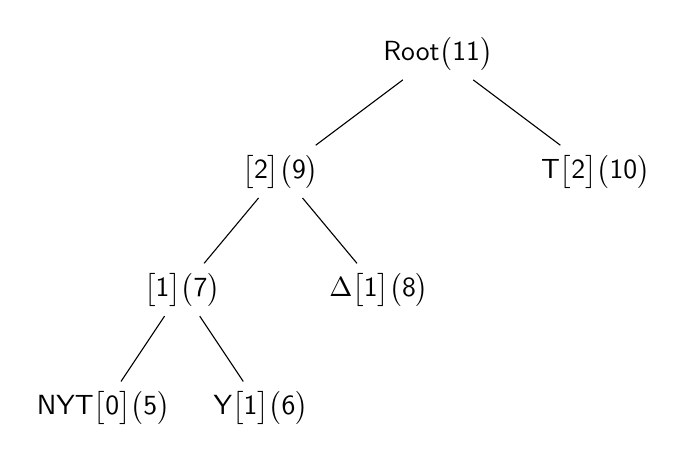
\begin{tikzpicture}[level 1/.style={sibling distance=4cm},level 2/.style={sibling distance=2.5cm},level 3/.style={sibling distance=2cm}]
	\node {Root\big(11\big)}
		child { node {\big[2\big]\big(9\big)}  
                child { node {\big[1\big]\big(7\big)}  
                            child{ node{NYT\big[0\big]\big(5\big)}}
                            child{ node{Y\big[1\big]\big(6\big)}}
                      }
                child{ node{$\Delta$\big[1\big]\big(8\big)}}
              }
         child {node{T\big[2\big]\big(10\big)}}	
	;
\end{tikzpicture}
\item Encode 1 = T.
\end{itemize}
$\therefore \text{final message}= T T \Delta Y T$.
\end{enumerate}
\end{solution}

\begin{question}
Use the Golomb code, with m=2, to code the above sequence.
\end{question}
\begin{solution}
\begin{tabular}{|c|c|c|c|c|c|c|c|c|}
\hline 
Symbol & A & C & A & C & T & A & N \\ 
\hline 
Code & 01 & 100 & 01 & 100 & 1100 & 01 & 101 \\ 
\hline 
\end{tabular} 
\end{solution}

\begin{question}
Code the above sequence using Move-To-Front.
\end{question}
\begin{solution}
\begin{tabular}{|c|c|c|c|c|c|c|c|c|}
\hline 
Symbol & A & C & A & C & T & A & N \\ 
\hline 
Code & 01 & 100 & 100 & 100 & 1100 & 101 & 1100 \\ 
\hline 
\end{tabular} 
\end{solution}

\begin{question}
Code the number 7 using.
\begin{enumerate}
\item Golomb code, with m=3.
\item Rice code, fundamental sequence.
\item Rice code, split sample option, with m=3, and k=5.
\end{enumerate}
\end{question}
\begin{solution}
\begin{enumerate}
\item 11010
\item 11111110
\item 1110
\end{enumerate}
\end{solution}

\begin{question}
Code the number 6. First, use Golomb code with m=3.
Next use Recursive indexing, with a
representation alphabet of size 3. Use variable
length code for entropy coding, with smaller
numbers having short length. Draw the VLC tree.
Label different parts of each code.

\end{question}
\begin{solution}
\begin{itemize}
\item Golomb code. q=2, r=0. Code = unary(2):prefix(0) = 1100
\item RI code. C(6)=$b_2b_2b_2b_0=00010$
\begin{tikzpicture}[level 1/.style={sibling distance=4cm},level 2/.style={sibling distance=2.5cm},level 3/.style={sibling distance=2cm}]
	\node {Root}
	    child {node{$b_2$}}	
		child { node {}  
                child{ node {$b_0$}}
                child{ node {$b_1$}}
              }
	;
\end{tikzpicture}

\end{itemize}
\end{solution}


\begin{question}
Using adaptive Huffman coding, code the string “COCOAC”. Show the development of the
coding tree. Assume that the used alphabet has only the 3 characters A, C, and O. Use VLC for new character coding.
\end{question}
\begin{solution}
Initial codes: \\
\begin{tabular}{|c|c|}
\hline 
A & 0 \\ 
\hline 
C & 10 \\ 
\hline 
O & 11 \\ 
\hline 
\end{tabular} \\

\begin{itemize}
\item Code C = 10. Transmit 10. \\
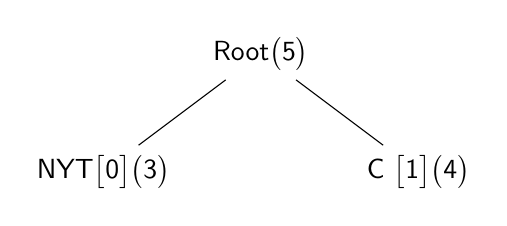
\begin{tikzpicture}[level 1/.style={sibling distance=4cm},level 2/.style={sibling distance=2.5cm},level 3/.style={sibling distance=2cm}]
	\node {Root\big(5\big)}
	    child { node{NYT\big[0\big]\big(3\big)}}	
		child { node{C  \big[1\big]\big(4\big)}}
	;
\end{tikzpicture} 
\item Code O = Code(NYT):Code(O). Transmit 011. \\
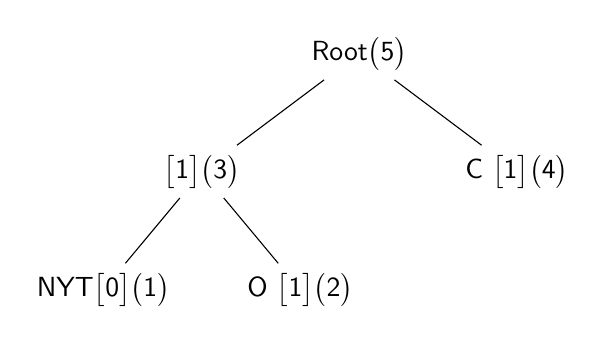
\begin{tikzpicture}[level 1/.style={sibling distance=4cm},level 2/.style={sibling distance=2.5cm},level 3/.style={sibling distance=2cm}]
	\node {Root\big(5\big)}
	    child { node{\big[1\big]\big(3\big)}
	            child { node{NYT\big[0\big]\big(1\big)}}	
		        child { node{O  \big[1\big]\big(2\big)}}}	
		child { node{C  \big[1\big]\big(4\big)}}
	;
\end{tikzpicture} 
\item Code C = 1. Transmit 1. \\
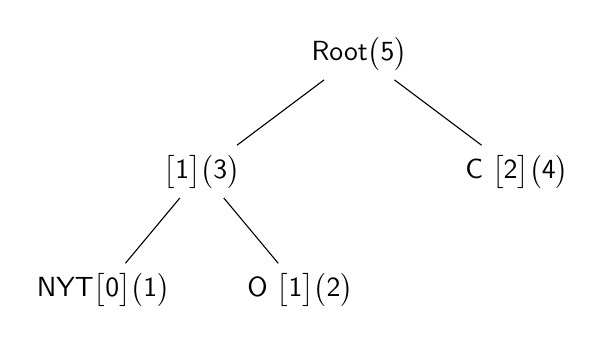
\begin{tikzpicture}[level 1/.style={sibling distance=4cm},level 2/.style={sibling distance=2.5cm},level 3/.style={sibling distance=2cm}]
	\node {Root\big(5\big)}
	    child { node{\big[1\big]\big(3\big)}
	            child { node{NYT\big[0\big]\big(1\big)}}	
		        child { node{O  \big[1\big]\big(2\big)}}}	
		child { node{C  \big[2\big]\big(4\big)}}
	;
\end{tikzpicture}
\item Code O = 01. Transmit 01. \\
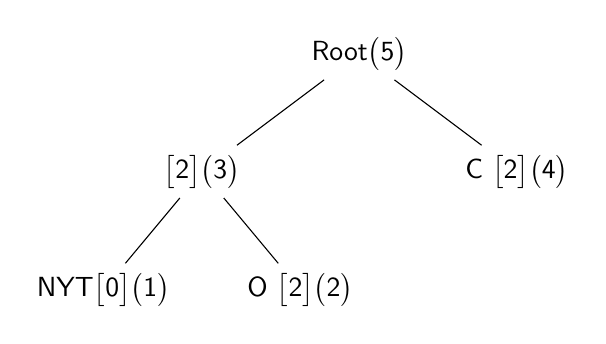
\begin{tikzpicture}[level 1/.style={sibling distance=4cm},level 2/.style={sibling distance=2.5cm},level 3/.style={sibling distance=2cm}]
	\node {Root\big(5\big)}
	    child { node{\big[2\big]\big(3\big)}
	            child { node{NYT\big[0\big]\big(1\big)}}	
		        child { node{O  \big[2\big]\big(2\big)}}}	
		child { node{C  \big[2\big]\big(4\big)}}
	;
\end{tikzpicture}
\item Code A = Code(NYT):Code(A). Transmit 000. \\
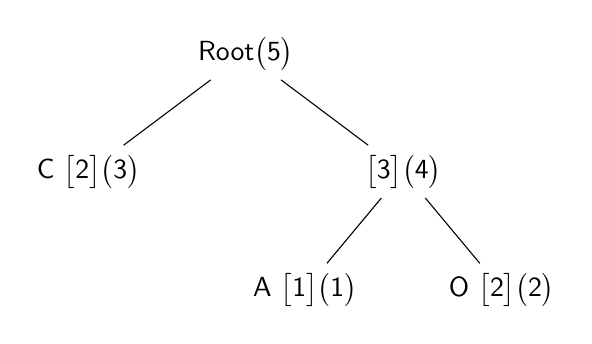
\begin{tikzpicture}[level 1/.style={sibling distance=4cm},level 2/.style={sibling distance=2.5cm},level 3/.style={sibling distance=2cm}]
	\node {Root\big(5\big)}
		child { node{C  \big[2\big]\big(3\big)}}
	    child { node{\big[3\big]\big(4\big)}
	            child { node{A  \big[1\big]\big(1\big)}}	
		        child { node{O  \big[2\big]\big(2\big)}}}	
	;
\end{tikzpicture}
\item Code C = 0. Transmit 0.
\end{itemize}
 $\therefore \text{final code}= 100111010000$
\end{solution}


\chapter*{Arithmetic Coding}


\begin{question}
Given the frequency counts shown: \\
\begin{tabular}{|c|c|c|c|}
\hline 
Symbol & A & C & G \\ 
\hline 
Count & 9 & 2 & 17 \\ 
\hline 
\end{tabular} \\
\begin{enumerate}
\item  What is the word length required for a digital arithmetic encoder to unambiguously encode the above symbols?
\item Calculate the cumulative count and the total count for the above symbols.
\end{enumerate}
\end{question}
\begin{solution}
\begin{enumerate}
\item 6 bits.
\item \begin{tabular}{|c|c|c|c|}
\hline 
Symbol & A & C & G \\ 
\hline 
Count & 9 & 11 & 28 \\ 
\hline 
\end{tabular} \\
\end{enumerate}
\end{solution}

\begin{question}
Using a word length of 8 bits, encode the symbols “CACG”. Use the table given below to report your results. Give l and u in binary form. Use E to identify the scale operation. Assume the given initial l \& u values, and initial scale3 = 4.
\end{question}
\begin{solution}
\begin{tabular}{|c|c|c|c|c|c|c|}
\hline 
Step & Symbol & l & u & E & s3 & Code \\ 
\hline 
n-1 & • & 00111111 & 11000001 & - & 4 & - \\ 
\hline 
n & C & 01101001 & 01110001 & E1 & 0 & 01111 \\ 
\hline 
• & • & 11010010 & 11100011 & E2.E2 & 0 & 11 \\ 
\hline 
• & • & 01001000 & 10001111 & E3 & 1 & - \\ 
\hline 
• & • & 00010000 & 10011111 & - & 1 & - \\ 
\hline 
n+1 & A & 00010000 & 00111101 & E1 & 0 & 01 \\ 
\hline 
• & • & 00100000 & 01111011 & E1 & 0 & 0 \\ 
\hline 
• & • & 01000000 & 11110111 & - & 0 & - \\ 
\hline 
n+2 & C & 01111011 & 10000111 & E3 & 1 & - \\ 
\hline 
• & • & 01110110 & 10001111 & E3 & 2 & - \\ 
\hline 
• & • & 01101100 & 10011111 & E3 & 3 & - \\ 
\hline 
• & • & 01011000 & 10111111 & E3 & 4 & - \\ 
\hline 
• & • & 00110000 & 11111111 & - & 4 & - \\ 
\hline 
n+3 & G & 10000001 & 11111111 & E2 & 0 & 10000 \\ 
\hline 
• & • & 00000010 & 11111111 & - & 0 & 00000000 \\ 
\hline 
\end{tabular} 
\end{solution}

\begin{question}
Using a word length of 8 bits, decode the first 5 symbols of the stream
“0111000100000111110010000001111001010101001010010101”. Use the table given below to
report your results. Give l and u in binary form. Use E to identify the scale operation. Assume the
given initial l \& u values, and initial scale3 = 4.
\end{question}
\begin{solution}
\begin{tabular}{|c|c|c|c|c|c|c|}
\hline 
Step & Symbol & l & u & tag & E & s3 \\ 
\hline 
n-1 & • & 00111111 & 11000001 & • & - & 4 \\ 
\hline 
n & C & 01101001 & 01110001 & 01110001 & E1 & 0 \\ 
\hline 
• & • & 11010010 & 11100011 & 11100010 & E2.E2 & 0 \\ 
\hline 
• & • & 01001000 & 10001111 & 10001000 & E3 & 1 \\ 
\hline 
• & • & 00010000 & 10011111 & 10010000 & - & 1 \\ 
\hline 
n+1 & G & 01001000 & 10011111 & 10010000 & E3 & 2 \\ 
\hline 
• & • & 00010000 & 10111111 & 10100000 & - & 2 \\ 
\hline 
n+2 & G & 01010101 & 10111111 & 10100000 & E3 & 3 \\ 
\hline 
• & • & 00101010 & 11111111 & 11000001 & - & 3 \\ 
\hline 
n+3 & G & 01111110 & 11111111 & 11000001 & - & 3 \\ 
\hline 
n+4 & G & 10110001 & 11111111 & 11000001 & E2 & 0 \\ 
\hline 
• & • & 01100010 & 11111111 & 10000011 & - & 0 \\ 
\hline 
n+5 & A & • & • & • & • & 0 \\ 
\hline 
\end{tabular} 
\end{solution}


\chapter*{Dictionary Methods}

\begin{question}

Given the sequence \{101011010010001001101010100101111111000000\}, use (LZ78/W/Y) to
encode/decode the first 7 phrases. Show the generated phrases, the corresponding code, and the encoder tree after each coding/decoding cycle. Use suppression, excision and prefix coding.

\end{question}
\begin{solution}
\begin{tabular}{|c|c|c|c|}
\hline 
• & LZ78 SEP & LZW EP & LZY SEP \\ 
\hline 
Phrase 1 & 1 & 1 & 1 \\ 
\hline 
Code 1 & 1 & 1 & 1 \\ 
\hline 
Phrase 2 & 0 & 0 & 0 \\ 
\hline 
Code 2 & 0 & 0 & 0 \\ 
\hline 
Phrase 3 & 10 & 10 & 10 \\ 
\hline 
Code 3 & 00 & 10 & 10 \\ 
\hline 
Phrase 4 & 11 & 1 & 01 \\ 
\hline 
Code 4 & 0 & 01 & 110 \\ 
\hline 
Phrase 5 & 01 & 101 & 1 \\ 
\hline 
Code 5 & 01 & 110 & 01 \\ 
\hline 
Phrase 6 & 00 & 0 & 101 \\ 
\hline 
Code 6 & 00 & 00 & 101 \\ 
\hline 
Phrase 7 & 100 & 01 & 01 \\ 
\hline 
Code 7 & 000 & 01 & 011 \\ 
\hline 
\end{tabular} 

\begin{enumerate}
\item LZ87 SEP Encoder \& Decoder
\begin{itemize}
\item \begin{tikzpicture}[level 1/.style={sibling distance=4cm},level 2/.style={sibling distance=2.5cm},level 3/.style={sibling distance=2cm}]
	\node {R}
	;
\end{tikzpicture} 

\item \begin{tikzpicture}[level 1/.style={sibling distance=4cm},level 2/.style={sibling distance=2.5cm},level 3/.style={sibling distance=2cm}]
	\node {R}
		child { }
	    child { node{1}}	
	;
\end{tikzpicture}
\item \begin{tikzpicture}[level 1/.style={sibling distance=4cm},level 2/.style={sibling distance=2.5cm},level 3/.style={sibling distance=2cm}]
	\node {R}
		child { node{2}}
	    child { node{1}}	
	;
\end{tikzpicture}
\item \begin{tikzpicture}[level 1/.style={sibling distance=4cm},level 2/.style={sibling distance=2.5cm},level 3/.style={sibling distance=2cm}]
	\node {R}
		child { node{2}}
	    child { node{1}
	        child { node{3}}	}	
	;
\end{tikzpicture}
\item \begin{tikzpicture}[level 1/.style={sibling distance=4cm},level 2/.style={sibling distance=2.5cm},level 3/.style={sibling distance=2cm}]
	\node {R}
		child { node{2}}
	    child { node{1}
	        child { node{3}}
	        child { node{4}} }	
	;
\end{tikzpicture}
\item \begin{tikzpicture}[level 1/.style={sibling distance=4cm},level 2/.style={sibling distance=2.5cm},level 3/.style={sibling distance=2cm}]
	\node {R}
		child { node{2}
		    child {} 
		    child { node{5}}    }
	    child { node{1}
	        child { node{3}}
	        child { node{4}}	}	
	;
\end{tikzpicture}
\item \begin{tikzpicture}[level 1/.style={sibling distance=4cm},level 2/.style={sibling distance=2.5cm},level 3/.style={sibling distance=2cm}]
	\node {R}
		child { node{2}
		    child { node{6}} 
		    child { node{5}}    }
	    child { node{1}
	        child { node{3}}
	        child { node{4}}	}	
	;
\end{tikzpicture}

\item \begin{tikzpicture}[level 1/.style={sibling distance=4cm},level 2/.style={sibling distance=2.5cm},level 3/.style={sibling distance=2cm}]
	\node {R}
		child { node{2}
		    child { node{6}} 
		    child { node{5}}    }
	    child { node{1}
	        child { node{3} 
	                    child{ node{7}} }
	        child { node{4}}	}	
	;
\end{tikzpicture}
\end{itemize}



\item LZW EP Tree
\begin{itemize}
\item  \begin{tikzpicture}[level 1/.style={sibling distance=4cm},level 2/.style={sibling distance=2.5cm},level 3/.style={sibling distance=2cm}]
	\node {R}
		child { node{0} }
	    child { node{1}	}	
	;
\end{tikzpicture}
\item  \begin{tikzpicture}[level 1/.style={sibling distance=4cm},level 2/.style={sibling distance=2.5cm},level 3/.style={sibling distance=2cm}]
	\node {R}
		child { node{0} }
	    child { node{1} 
	            child{ node{2}	} }	
	;
\end{tikzpicture}
\item \begin{tikzpicture}[level 1/.style={sibling distance=4cm},level 2/.style={sibling distance=2.5cm},level 3/.style={sibling distance=2cm}]
	\node {R}
		child { node{0} 
		        child{} 
		        child{ node{3}} } 
	    child { node{1} 
	            child{ node{2}} }	
	;
\end{tikzpicture}
\item \begin{tikzpicture}[level 1/.style={sibling distance=4cm},level 2/.style={sibling distance=2.5cm},level 3/.style={sibling distance=2cm}]
	\node {R}
		child { node{0} 
		        child{} 
		        child{ node{3}} }
	    child { node{1} 
	            child{ node{2}	
	                    child{}
	                    child{ node {4} }} }	
	;
\end{tikzpicture}

\item \begin{tikzpicture}[level 1/.style={sibling distance=4cm},level 2/.style={sibling distance=2.5cm},level 3/.style={sibling distance=2cm}]
	\node {R}
		child { node{0} 
		        child{} 
		        child{ node{3}} } 
	    child { node{1} 
	            child{ node{2}
	                    child{}
	                    child{ node {4} }	} 
	            child{ node{5} } }	
	;
\end{tikzpicture}
\item \begin{tikzpicture}[level 1/.style={sibling distance=4cm},level 2/.style={sibling distance=2.5cm},level 3/.style={sibling distance=2cm}]
	\node {R}
		child { node{0} 
		        child{} 
		        child{ node{3}} } 
	    child { node{1} 
	            child{ node{2}
	                    child{}
	                    child{ node {4} 
	                            child{  node{6} } }	} 
	            child{ node{5} } }	
	;
\end{tikzpicture}

\item  \begin{tikzpicture}[level 1/.style={sibling distance=4cm},level 2/.style={sibling distance=2.5cm},level 3/.style={sibling distance=2cm}]
	\node {R}
		child { node{0} 
		        child{ node{7}} 
		        child{ node{3}} } 
	    child { node{1} 
	            child{ node{2}
	                    child{}
	                    child{ node {4} 
	                            child{  node{6} } }	} 
	            child{ node{5} } }	
	;
\end{tikzpicture}

\end{itemize}


\item LZY SEP 
\begin{itemize}
\item  \begin{tikzpicture}[level 1/.style={sibling distance=4cm},level 2/.style={sibling distance=2.5cm},level 3/.style={sibling distance=2cm}]
	\node {R}
		child { node{0} }
	    child { node{1}	}	
	;
\end{tikzpicture}
\item  \begin{tikzpicture}[level 1/.style={sibling distance=4cm},level 2/.style={sibling distance=2.5cm},level 3/.style={sibling distance=2cm}]
	\node {R}
		child { node{0} }
	    child { node{1} 
	            child{ node{2}	} }	
	;
\end{tikzpicture}
\item \begin{tikzpicture}[level 1/.style={sibling distance=4cm},level 2/.style={sibling distance=2.5cm},level 3/.style={sibling distance=2cm}]
	\node {R}
		child { node{0} 
		        child{} 
		        child{ node{3}} } 
	    child { node{1} 
	            child{ node{2}} }	
	;
\end{tikzpicture}
\item \begin{tikzpicture}[level 1/.style={sibling distance=4cm},level 2/.style={sibling distance=2.5cm},level 3/.style={sibling distance=2cm}]
	\node {R}
		child { node{0} 
		        child{} 
		        child{ node{3}} }
	    child { node{1} 
	            child{ node{2}	
	                    child{}
	                    child{ node {4} }} }	
	;
\end{tikzpicture}

\item \begin{tikzpicture}[level 1/.style={sibling distance=4cm},level 2/.style={sibling distance=2.5cm},level 3/.style={sibling distance=2cm}]
	\node {R}
		child { node{0} 
		        child{} 
		        child{ node{3} 
		                child{ node{}}
		                child{ node{5}} } }
	    child { node{1} 
	            child{ node{2}	
	                    child{}
	                    child{ node {4} }} }	
	;
\end{tikzpicture}

\item \begin{tikzpicture}[level 1/.style={sibling distance=4cm},level 2/.style={sibling distance=2.5cm},level 3/.style={sibling distance=2cm}]
	\node {R}
		child { node{0} 
		        child{} 
		        child{ node{3} 
		                child{ node{}}
		                child{ node{5}} } }
	    child { node{1} 
	            child{ node{2}	
	                    child{}
	                    child{ node {4} 
	                            child{ node{7}} }} }	
	;
\end{tikzpicture}

\end{itemize}
\end{enumerate}
\end{solution}

\begin{question}
Using LZ77 (Tail biting, Future), encode, in binary, the first four phrases following the underlined
window. Indicate the meaning of each part of the code, e.g. new character, Length, ...etc.
\underline{011001001111010001001111110110011101110} \\
1000100111111001100111011101001110001001111000111000001111
\end{question}
\begin{solution}
\begin{enumerate}
\item First Phrase: 100010011111100 \\ 
Current Win=011001001111010001001111110110011101110 \\
Code= 00110101110\\
New Win=011001001111010001001111110\\110011101110100010011111100 \\
Stream=110001001111000111000001111

\item Second Phrase: 1100111011101001 \\
Current Win=011001001111010001001111110110011101110100010011111100 \\
Code= 01101101110\\
New Win=0110010011110100010011111101100\\111011101000100111111001100111011101001 \\
Stream=110001001111000111000001111

\item Third Phrase: 11000 \\
Current Win=01100100111101000100111111011001\\11011101000100111111001100111011101001 \\
Code= 0110110 0011\\
New Win=0110010011110100010011111101100111\\01110100010011111100110011101110100111000 \\
Stream=1001111000111000001111

\item Fourth Phrase=100111100 \\
Current Win=011001001111010001001111110110011\\101110100010011111100110011101110100111000 \\
Code= 00001010000111\\
New Win=011001001111010001001111110110011101110\\100010011111100110011101110100111000100111100 
 
\end{enumerate}
\end{solution}

\begin{question}
Code the first 6 phrases of the sequence {101101101110010010111111001...}. Use LZ77. Show the generated phrases, the corresponding code, and the search window after each coding cycle.
\end{question}
\begin{solution}
\begin{tabular}{|c|c|c|c|}
\hline 
i & Phrase & Code & Window \\ 
\hline 
1 & 1 & 1 & 1 \\ 
\hline 
2 & 0 & 10 & 10 \\ 
\hline 
3 & 11 & 001 & 1011 \\ 
\hline 
4 & 0110 & 01110 & 10110110 \\ 
\hline 
5 & 111 & 101101 & 10110110111 \\ 
\hline 
6 & 00 & 1011000 & 1011011011100 \\ 
\hline 
\end{tabular} 
\end{solution}



\chapter*{Predictive}

\begin{question}
Use ppm technique, and the following probabilities. Show the different context tables after coding the sequence “AGAAGT”. Assume max context of 2.

\end{question}
\begin{solution}
\begin{enumerate}
\item -1 order context. \\
\begin{tabular}{|c|c|c|}
\hline 
Letter  & Count & CumCount \\ 
\hline 
A & 1 & 1 \\ 
\hline 
C & 1 & 2 \\ 
\hline 
G & 2 & 4 \\ 
\hline 
T & 4 & 8 \\ 
\hline 
\end{tabular} 
\item zero order context. \\
\begin{tabular}{|c|c|c|}
\hline 
Letter  & Count & CumCount \\ 
\hline 
A & 3 & 1 \\ 
\hline 
C & 2 & 2 \\ 
\hline 
T & 1 & 4 \\ 
\hline 
Esc & 1 & 8 \\ 
\hline 
\end{tabular} 
\item first order context. \\
\begin{tabular}{|c|c|c|c|}
\hline 
Context & Letter & Count & CumCount \\ 
\hline 
A & G & 2 & 2 \\ 
\hline 
• & A & 1 & 3 \\ 
\hline 
• & Esc & 1 & 4 \\ 
\hline 
G & A & 1 & 1 \\ 
\hline 
• & T & 1 & 2 \\ 
\hline 
• & Esc & 1 & 3 \\ 
\hline 
\end{tabular} 
\item second order context. \\
\begin{tabular}{|c|c|c|c|}
\hline 
Context & Letter & Count & CumCount \\ 
\hline 
AG & A & 1 & 1 \\ 
\hline 
• & T & 1 & 2 \\ 
\hline 
• & Esc & 1 & 3 \\ 
\hline 
GA & A & 1 & 1 \\ 
\hline 
• & Esc & 1 & 2 \\ 
\hline 
AA & G & 1 & 1 \\ 
\hline 
• & Esc & 1 & 2 \\ 
\hline \hline 

\end{tabular} 


\end{enumerate}
\end{solution}

\begin{question}
The sequence “CAGT” is encoded. Show the generated counts and the cumulative counts.
Modify the above context tables during coding. Use the exclusion principle.
\end{question}
\begin{solution}
\begin{tabular}{|c|c|c|}
\hline 
Letter & Count & CumCount \\ 
\hline 
C & 1 & 2 \\ 
\hline 
A & 3 & 3 \\ 
\hline 
G & 2 & 2 \\ 
\hline 
T & 1 & 2 \\ 
\hline 
\end{tabular}  \\


Updated Tables:
\begin{enumerate}
\item -1 order context. \\
\begin{tabular}{|c|c|c|}
\hline 
Letter  & Count & CumCount \\ 
\hline 
A & 1 & 1 \\ 
\hline 
C & 2 & 3 \\ 
\hline 
G & 4 & 7 \\ 
\hline 
T & 5 & 12 \\ 
\hline 
\end{tabular} 
\item zero order context. \\
\begin{tabular}{|c|c|c|}
\hline 
Letter  & Count & CumCount \\ 
\hline 
A & 4 & 4 \\ 
\hline 
C & 1 & 5 \\ 
\hline 
G & 3 & 8 \\ 
\hline 
T & 2 & 10 \\ 
\hline 
Esc & 1 & 11 \\ 
\hline 
\end{tabular} 
\item first order context. \\
\begin{tabular}{|c|c|c|c|}
\hline 
Context & Letter & Count & CumCount \\ 
\hline 
A & G & 3 & 3 \\ 
\hline 
• & A & 1 & 4 \\ 
\hline 
• & Esc & 1 & 5 \\ 
\hline 
T & C & 1 & 1 \\ 
\hline 
• & Esc & 1 & 2 \\ 
\hline 
C & A & 1 & 1 \\ 
\hline 
• & Esc & 1 & 2 \\ 
\hline 
\end{tabular} 
\item second order context. \\
\begin{tabular}{|c|c|c|c|}
\hline 
Context & Letter & Count & CumCount \\ 
\hline 
AG & A & 1 & 1 \\ 
\hline 
• & T & 2 & 3 \\ 
\hline 
• & Esc & 1 & 1 \\ 
\hline 
GA & A & 1 & 2 \\ 
\hline 
• & Esc & 1 & 3 \\ 
\hline 
AA & G & 1 & 1 \\ 
\hline 
• & Esc & 1 & 2 \\ 
\hline 
GT & C & 1 & 1 \\ 
\hline 
• & Esc & 1 & 2 \\ 
\hline 
TC & A & 1 & 1 \\ 
\hline 
• & Esc & 1 & 2 \\ 
\hline 
CA & G & 1 & 1 \\ 
\hline 
• & Esc & 1 & 2 \\ 
\hline 
\end{tabular} 


\end{enumerate}




\end{solution}


\begin{question}
Using Burrows-Wheeler transform, and the alphabet \{ A, C, T, N, $\Delta$ \}:
Code the sequence \{ACACAT\}. Let row index start at 0.
\end{question}
\begin{solution}
\begin{enumerate}
\item Permutations \\
A C A C A T \\
C A C A T A \\
A C A T A C \\
C A T A C A \\
A T A C A C \\
T A C A C A 
\item Sorted Permutations \\ 
A C A C A T \\
A C A T A C \\
A T A C A C \\
C A C A T A \\
C A T A C A \\
T A C A C A \\ 
\item First row idx=0. Last column=\{TCCAAA\}. \\
Code = Prefix(0):MTF(TCCAAA).
\end{enumerate}
\end{solution}


\begin{question}
Find the Move to Front code for the sequence \{$N N \Delta \Delta \Delta N$\}.
\end{question}
\begin{solution}
\begin{tabular}{|c|c|c|c|c|}
\hline 
0 & 1 & 2 & 3 & 4 \\ 
\hline 
A & C & T & N & $\Delta$ \\ 
\hline 
N & A & C & T & $\Delta$ \\ 
\hline 
$\Delta$ & N & A & C & T \\ 
\hline 
N & $\Delta$ & A & C & T \\ 
\hline 
\end{tabular} \\
Code=\{3,0,4,0,0,1\}
\end{solution}


\begin{question}
Find the inverse Burrows Wheeler transform of \{3, CNACAAA\}. Row numbers are given
at the left most column.
\end{question}
\begin{solution}
\begin{tabular}{|c|c|c|c|c|c|c|c|}
\hline 
0 & A & • & • & • & • & • & C \\ 
\hline 
1 & A & • & • & • & • & • & N \\ 
\hline 
2 & A & • & • & • & • & • & A \\ 
\hline 
3 & A & N & A & C & A & A & C \\ 
\hline 
4 & C & • & • & • & • & • & A \\ 
\hline 
5 & C & • & • & • & • & • & A \\ 
\hline 
6 & N & • & • & • & • & • & A \\ 
\hline 
\end{tabular} \\
Decoded sequence: ANACAAC. 
\end{solution}

\begin{question}
Assume that the underlined part of the sequence “\underline{ACGACGA}CATGCGA” has already been encoded. Encode next 2 phrases using the Associative Coder of Buyanovsky (ACB).
\end{question}
\begin{solution}
\begin{tabular}{|c|c|c|}
\hline 
Unsorted & • & Sorted \\ 
\hline 
A|CGACGA & 1 & A|CGACGA \\ 
\hline 
AC|GACGA & 2 & ACGA|CGA \\ 
\hline 
ACG|ACGA & 3 & AC|GACGA \\ 
\hline 
ACGA|CGA & 4 & ACGAC|GA \\ 
\hline 
ACGAC|GA & 5 & ACG|ACGA \\ 
\hline 
ACGACG|A & 6 & ACGACG|A \\ 
\hline 
\end{tabular} \\
The best context match between 1 and 2. \\
The best match of content: 2 \\
Output (2-1,1,’A’) \\ \\
\begin{tabular}{|c|c|c|}
\hline 
Unsorted & • & Sorted \\ 
\hline 
A|CGACGACA & 1 & A|CGACGACA \\ 
\hline 
AC|GACGACA & 2 & ACGA|CGACA \\ 
\hline 
ACG|ACGACA & 3 & ACGACGA|CA \\ 
\hline 
ACGA|CGACA & 4 & AC|GACGACA \\ 
\hline 
ACGAC|GACA & 5 & ACGAC|GACA \\ 
\hline 
ACGACG|ACA & 6 & ACGACGAC|A \\ 
\hline 
ACGACGA|CA & 7 & ACG|ACGACA \\ 
\hline 
ACGACGAC|A & 8 & ACGACG|ACA \\ 
\hline 
\end{tabular} \\
The best context match between 1 and 3. \\
The best match of content: none \\
Output (0,0,’T’).

\end{solution}



\end{document}


